\documentclass[a4paper]{article}
\usepackage[utf8]{inputenc}
\usepackage[russian,english]{babel}
\usepackage[T2A]{fontenc}
\usepackage[left=10mm, top=20mm, right=18mm, bottom=15mm, footskip=10mm]{geometry}
\usepackage{indentfirst}
\usepackage{amsmath,amssymb}
\usepackage[italicdiff]{physics}
\usepackage{graphicx}
\usepackage{caption}
\usepackage{float}
\renewcommand{\thefootnote}{\fnsymbol{footnote}}
\usepackage{tablefootnote}
\usepackage{footmisc}
\usepackage[parfill]{parskip}
\usepackage[utf8]{inputenc}\newcommand{\approxtext}[1]{\ensuremath{\stackrel{\text{#1}}{\approx}}}
\graphicspath{{images/}}
\DeclareGraphicsExtensions{.pdf,.png,.jpg}
\usepackage{wrapfig}
\captionsetup{labelformat=empty}
\usepackage{caption}
\captionsetup[figure]{name=Рисунок}
\captionsetup[table]{name=Таблица}
  
\title{\textbf{Отчет о выполненой лабораторной работе 2.5.1}}
\date{}
\author{Котляров Михаил, Б01-402}

\begin{document}

\maketitle
	
	\section{Введение}
	
	\textbf{Цель работы:} 1) измерение диаметра иглы с помощью известного коэффициента поверхностного натяжения спирта, измерение температурной зависимости коэффициента поверхностного натяжения дистиллированной воды  2) определение полной поверхностной энергии  и теплоты, необходимой для изотермического образования единицы  поверхности жидкости  при различной температуре. \\
	\textbf{Оборудование:} прибор Ребиндера с термостатом и микроманометром; исследуемые жидкости; стаканы с дистиллированной водой, шприц для промывания; микроскоп; линейка.
	
	\section{Теоретические сведения}
\begin{enumerate}
\item \textbf{Термодинамика поверхностного натяжения.}\\
Работа, необходимая для обратимого изотермического образования единицы площади поверхности жидкости, называется коэффициентом поверхностного натяжения и обозначается $\sigma$.
Коэффициент поверхностного натяжения равен силе, действующей на единицу длины контура поверхности жидкости. Эта сила направлена вдоль поверхности перпендикулярно линии контура.
\begin{equation*}
	\sigma = \frac{f}{L}.
	\eqno(1)
\end{equation*}
Из первого и второго начал термодинамики имеем:
\begin{equation*}
	\delta Q = dU + \delta A,
	\eqno(2)
\end{equation*}
\begin{equation*}
	dS = \frac{\delta Q}{T},
	\eqno(3)
\end{equation*}
где $dS$ - энтропия, функцией состояния, и поэтому является полным дифференциалом.
Работа по увеличению площади поверхностни жидкости на величину $d\Pi$ внешними силами равна $\sigma d\Pi$ по определению. Соответственно работа поверхностного слоя жидкости равна $\delta A = -\sigma d\Pi$. Используя первое и второе начала термодинамики получаем
\begin{equation*}
	\delta Q = dU_{\text{п}}-\sigma d\Pi,
\end{equation*}
\begin{equation*}
	dU_{\text{п}} = TdS + \sigma d\Pi,
	\eqno(4)
\end{equation*}
где $dU_{\text{п}}$ - полная поверхностная энергия.
Введем в эту формулу свободную энергию $\Psi_{\text{п}}$, равную по поределению
\begin{equation*}
	\Psi_{\text{п}} = U_{\text{п}} - TS.
	\eqno(5)
\end{equation*}
Тогда получим
\begin{equation*}
	d\Psi_{\text{п}} = dU_{\text{п}} - SdT - TdS = TdS + \sigma d\Pi - SdT - TdS = -SdT + \sigma d\Pi.
	\eqno(6)
\end{equation*}
Это соотношение между полными дифференциалами, поэтому 
\begin{equation*}
	S = - (\frac{\partial \Psi_{\text{п}}}{\partial T})_{\Pi},
	\eqno(7)
\end{equation*}
\begin{equation*}
	\sigma = (\frac{\partial \Psi_{\text{п}}}{\partial \Pi})_{T}.
	\eqno(8)
\end{equation*}
Интегрируя последнюю формулу, полагая, что при $\Psi_{\text{п}} = 0$, $\Pi = 0$, получаем
\begin{equation*}
	\Psi_{\text{п}} = \sigma \Pi.
	\eqno(9)
\end{equation*}

Подставив в (7), получим
\begin{equation*}
	S = -\Pi\frac{d\sigma}{dT}.
	\eqno(10)
\end{equation*}
Находим из (5) и (9) полную поверхностную энергию
\begin{equation*}
	U_{\text{п}} = (\sigma - T\frac{d\sigma}{dT})\Pi.
	\eqno(11)
\end{equation*}
По первому начлау термодинамики для увеличения площади поверхности нужно подвести тепло
\begin{equation*}
	Q = \Delta U_{\text{п}} - \sigma \Delta \Pi = -T\frac{d\sigma}{dT}\Delta \Pi.
	\eqno(12)
\end{equation*}
Следовательно, на единицу площади подведенное тепло равно
\begin{equation*}
	q  = -T\frac{d\sigma}{dT}.
	\eqno(13)
\end{equation*}
\item \textbf{Давление под изогнутой поверхностью жидкости.}\\
В общем случае нужно провести две взаимно перпендикулярные плоскости через нормаль к поверхности и найти у полученных в сечении линии радиусы соприкасающихся окружностей $r_1$ и $r_2$. Тогда
\begin{equation*}
	\Delta P = \sigma(\frac{1}{r_1} + \frac{1}{r_2}).
	\eqno(14)
\end{equation*}
Эта формула называется формулой Лапласа. В частности для сферической поверхности радиуса $r$ получим
\begin{equation*}
	\Delta P = P_{\text{внутри}} - P_{\text{снаружи}}= \frac{2\sigma}{r}.
	\eqno(15)
\end{equation*}
\end{enumerate}
\section{Экспериментальная установка}
Исследуемая жидкость (дистиллированная вода) наливается в сосуд (колбу) В (рис.1). Тестовая жидкость  (этиловый спирт) наливается  в сосуд Е.  При измерениях  колбы герметично закрываются  пробками.   Через одну из двух пробок  проходит полая металлическая игла С. Этой пробкой закрывается сосуд, в котором  проводятся измерения. Верхний конец иглы открыт в атмосферу, а нижний погружен в жидкость. Другой сосуд герметично закрывается второй пробкой. При создании достаточного  разряжения воздуха в колбе с иглой пузырьки воздуха начинают пробулькивать через жидкость. Поверхностное натяжение можно определить по величине разряжения $\Delta P$ (1), необходимого для прохождения пузырьков (при известном радиусе иглы). 

Разряжение в системе создается с помощью аспиратора А. Кран К2 разделяет две полости аспиратора. Верхняя полость при закрытом кране К2  заполняется водой. Затем кран К2 открывают и заполняют водой  нижнюю полость  аспиратора.  Разряжение воздуха создается в нижней полости  при открывании крана К1, когда  вода вытекает из неё по каплям. В колбах В и С, соединённых трубками с нижней полостью аспиратора,  создается такое же пониженное давление. Разность давлений в полостях с разряженным воздухом и атмосферой измеряется спиртовым микроманометром (устройство микроманометра описано в Приложении).  

Для стабилизации температуры исследуемой жидкости через рубашку D колбы В непрерывно прогоняется вода из термостата. 
\begin{figure}[H]
        \centering
        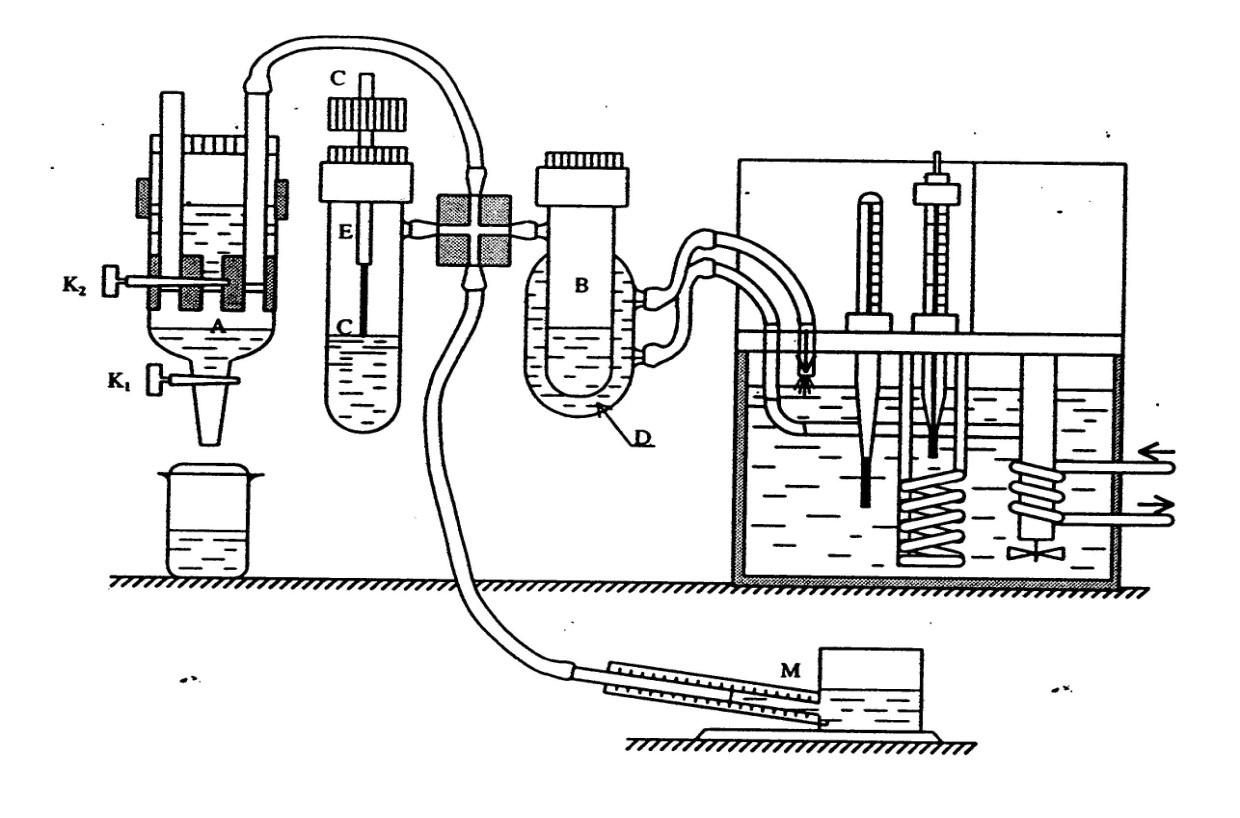
\includegraphics[scale=0.8]{Pictures/pic1.jpg}
        \caption{
        Схема установки для измерения температурной зависимости 
        коэффициента поверхностного натяжения
        }
 \end{figure} 
Обычно кончик иглы лишь касается поверхности жидкости, чтобы исключить влияние гидростатического давления столба жидкости. Однако при измерении температурной зависимости коэффициента поверхностного натяжения возникает ряд сложностей. Во-первых, большая теплопроводность металлической трубки приводит к тому, что температура на конце трубки заметно ниже, чем в глубине жидкости. Во-вторых, тепловое расширение поднимает уровень жидкости при увеличении температуры.  

Обе погрешности можно устранить, погрузив кончик трубки до самого дна. Полное давление, измеренное при этом микроманометром, $P = \Delta P + \rho gh$. Заметим, что $\rho gh$ от температуры практически не зависит, так как подъём уровня жидкости компенсируется уменьшением её плотности (произведение $\rho h$ определяется массой всей жидкости и поэтому постоянно). Величину  $\rho gh$ следует измерить двумя способами. Во-первых, замерить величину $P_1= \Delta P'$, когда кончик трубки только касается поверхности жидкости. Затем при этой же температуре опустить иглу до дна и замерить $Р_2= \rho gh + \Delta P"$ ($\Delta P'$, $\Delta P''$ – давление Лапласа). Из-за  несжимаемости  жидкости можно положить $\Delta P' = \Delta P''$ и тогда $\rho gh = P_2-P_1$. Во-вторых, при измерениях $Р_1$ и $Р_2$ замерить линейкой  глубину погружения иглы $h$. Это можно сделать, замеряя расстояние между верхним концом иглы и любой неподвижной частью прибора при положении иглы на поверхности и в глубине колбы. 

\section{Приборы и данные}
\begin{itemize}
    \item Микроманометр ММН-2400(5)-1б0, погрешность 6 Па.
    \item Микроскоп, погрешность 0,05 мм.
    \item Термостат LT 100, погрешность измерения температуры 1,5 К.
    \item Линейка, погрешность 0,5 мм.
\end{itemize}

\section{Выполнение}
\begin{enumerate}
\item Убедившись в герметичности, начнем измерения. Откроем кран К1. Подберем частоту падения капель из аспиратора так, чтобы максимальное давление микроманометра не зависело от этой частоты (не чаще, чем 1 капля в 5 секунд)
\item Измерим максимальное давление $\Delta P_{\text{спирт}} = C \times h \times K \times 9,80655 \times \frac{\gamma_{\text{спирт в манометре}}}{\gamma_{\text{исслед. жид.}}}$ при пробулькивании пузырьков воздуха через спирт ($C = 1,00; K = 0,2; \gamma_{\text{спирт в манометре}} = 0,81351 \text{ } \frac{\text{г}}{\text{см}^3}$, h - количество делений на шкале манометра). По разбросу результатов оценим случайную погрешность измерения.

\begin{table}[h!] 
	\caption{Таблица №1 Измерение максимального давления $\Delta P_{\text{спирт}}$}
	\begin{center}
		\begin{tabular}{|*{3}{c|}}
			\hline
			\textnumero  & $h$ & $\Delta P$, \text{Па} \\ \hline
			1&	$51 \pm 3$&	$100,03\pm 6$\\ \hline
			2&$51 \pm 3$&	$100,03\pm 6$\\ \hline
			3&	$50 \pm 3$&	$98,07\pm 6$\\ \hline
			4&	$51 \pm 3$&	$100,03\pm 6$\\ \hline
			5&	$51 \pm 3$&	$100,03\pm 6$\\ \hline
		\end{tabular}
	\end{center}
\end{table}
Получаем $\langle \Delta P\rangle = 99,64 $ Па, $\sigma_{\Delta P}^{\text{случ}} = 0,88$ Па, полная погрешность давления $\sigma_{\Delta P} = 6,01 (\varepsilon_{\Delta P} = 6,0 \%)$. По табличному значению коэффициенту поверхностного натяжения спирта $\sigma_{\text{спирта}} = 22,78 \frac{\text{мН}}{\text{м}}$ и формуле (15) рассчитаем диаметр иглы
\begin{equation*}
	\sigma_{d} = \frac{4 \sigma_{\text{спирта}} \sigma_{\Delta P}}{{\Delta P}^2}=0,055 \text{мм}
\end{equation*}
\begin{equation*}
	d_{\text{иглы}}^{exp} = \frac{4 \sigma_{\text{спирта}}}{{\Delta P}}=0,915 \pm 0,055 \text{ мм }(\varepsilon_{d} = 6,0\%)
\end{equation*}
Диаметр, измеренный на микроскопе равен $d = 1,10 \pm 0,05 \text{ мм}$ ($\varepsilon = 4,5\%$)

\item Промоем иглу 3 раза дистиллированной водой и перенесем в колбу с ней. Измерим максимальное давление $P_1$ при пробулькивании пузырьков, когда игла лишь касается поверхности воды.

\begin{table}[h!] 
	\caption{Таблица №2 Измерение максимального давления $\Delta P_{1}$ на поверхности}
	\begin{center}
		\begin{tabular}{|*{3}{c|}}
			\hline
			\textnumero  & $h$ & $\Delta P_1$, \text{Па} \\ \hline
			1&	$129 \pm 3$&	$206,15 \pm 6$\\ \hline
			2&	$129 \pm 3$&	$206,15 \pm 6$\\ \hline
			3&	$129 \pm 3$&	$206,15 \pm 6$\\ \hline
			4&	$127,5\pm 3$&	$203,75 \pm 6$\\ \hline
			5&	$128,5\pm 3$&	$205,35 \pm 6$\\ \hline
			6&	$129 \pm 3$&	$206,15 \pm 6$\\ \hline
		\end{tabular}
	\end{center}
\end{table}
Среднее давление $\langle \Delta P_1\rangle = 205,51 $ Па, $\sigma_{\Delta P}^{\text{случ}} = 0,40$ Па. 
Расстояние от верхней точки крышки с иглой до закручивающего элемента, измеренное линейкой, равно $H_1 = 2,25 \pm 00,5\text{ см}$.

\item Утопим иглу практически до самого дна.
\begin{table}[h!] 
	\caption{Таблица №3 Измерение максимального давления $\Delta P_{2}$ на дне}
	\begin{center}
		\begin{tabular}{|*{3}{c|}}
			\hline
			\textnumero  & $h$ & $\Delta P_2$, \text{Па} \\ \hline
			1&	$215 \pm 3$&	$297,24 \pm 6$\\ \hline
			2&	$215 \pm 3$&	$297,24 \pm 6$\\ \hline
			3&	$215 \pm 3$&	$297,24 \pm 6$\\ \hline
		\end{tabular}
	\end{center}
\end{table}
Среднее давление $\langle \Delta P_2\rangle = 297,24 $ Па. $ H_2 = 0,65 \pm 00,5$ см. \newline Таким образом рассчитаем $\Delta H$ и сравним с измеренным значением\\

\begin{equation*}
	\sigma_{H} = \frac{2\sigma_{P}}{\rho_{\text{воды}}g} = 0,12\text{ см},
\end{equation*}
\begin{equation*}
	\Delta H^{exp} = \frac{\Delta P_2 - \Delta P_1}{\rho_{\text{воды}}g} \approx 0,94 \pm 0,12 \text{ см}(\varepsilon = 13,1 \%).
\end{equation*}
\begin{equation*}
	\Delta H^{real} = H_1 - H_2 = 1,60 \pm 0,05 \text{ см},
\end{equation*}
Значительное расхождение в значениях можно объяснить тем, что возможно игла была загрязнена. Также температуры спирта и иглы не одинаковые. 

\item Включим термостат и подождем, пока температура для первой серии измерений установится. После этого подождем 5-7 минут для того, что исследуемая жидкость успела нагреться. Теперь проведем измерение давлений через каждые $5 ^\circ C$ c 20 до 60 $^\circ C$.
\begin{table}[h!] 
	\caption{Таблица №4 Измерение $\Delta P$ от температуры }
	\begin{center}
		\begin{tabular}{|*{7}{c|}}
			\hline
			 $T$, K & Плотность воды\footnotemark[1], $\frac{\text{г}}{\text{см}^2}$&$\langle h\rangle$ & $\langle \Delta P\rangle$, \text{Па} & $\sigma, \frac{\text{мН}}{\text{м}}$ & $\Delta \sigma, \frac{\text{мН}}{\text{м}}$ & $\varepsilon_{\sigma}$, \% \\ \hline
			$292,3\pm 1,5$& 0,99843 &	$215\pm 3$&	$297,24\pm6$&	81,74&	4,54&	5,55\\ \hline
			$298,5\pm 1,5$& 0,99707 &	$213\pm 3$&	$291,25\pm6$&	80,09&	4,47&	5,58\\ \hline
			$303,4\pm 1,5$& 0,99567 &	$212\pm 3$&	$288,45\pm6$&	79,32&	4,43&	5,59\\ \hline
			$308,1\pm 1,5$&0,99406  &	$211\pm 3$&	$285,71\pm6$&	78,57&	4,40&	5,60\\ \hline
			$313,1\pm 1,5$& 0,99225 &	$211\pm 3$&	$283,01\pm6$&	77,83&	4,36&	5,61\\ \hline
			$318,2\pm 1,5$& 0,99025 &	$210\pm 3$&	$280,36\pm6$&	77,10&	4,33&	5,62\\ \hline
			$323,0\pm 1,5$   & 0,9881   &	$208\pm 3$&	$277,74\pm6$&	76,38&	4,30&	5,63\\ \hline
			$329,2\pm 1,5$& 0,9853   &	$205\pm 3$&	$275,29\pm6$&	75,71&	4,27&	5,64\\ \hline
			$333,0\pm 1,5$   & 0,9832   &	$204\pm 3$&	$271,01\pm6$&	74,53&	4,21&	5,65\\ \hline
		\end{tabular}
	\end{center}
\end{table}
\footnotetext[1]{Данные для измерений с 1 по 4 взяты из книги Лабораторный практикум по общей физике Том 1 Термодинамика и молекулярная физика, остальные с сайта in-chemistry.ru, ссылка https://in-chemistry.ru/plotnost-vody-v-zavisimosti-ot-temperatury-tablitsa}
\item Построим по МНК график зависимости $\sigma(T)$ и определим по нему температурный коэффициент $\frac{d\sigma}{dT}$.
\clearpage
\begin{figure}[h!]
\centering{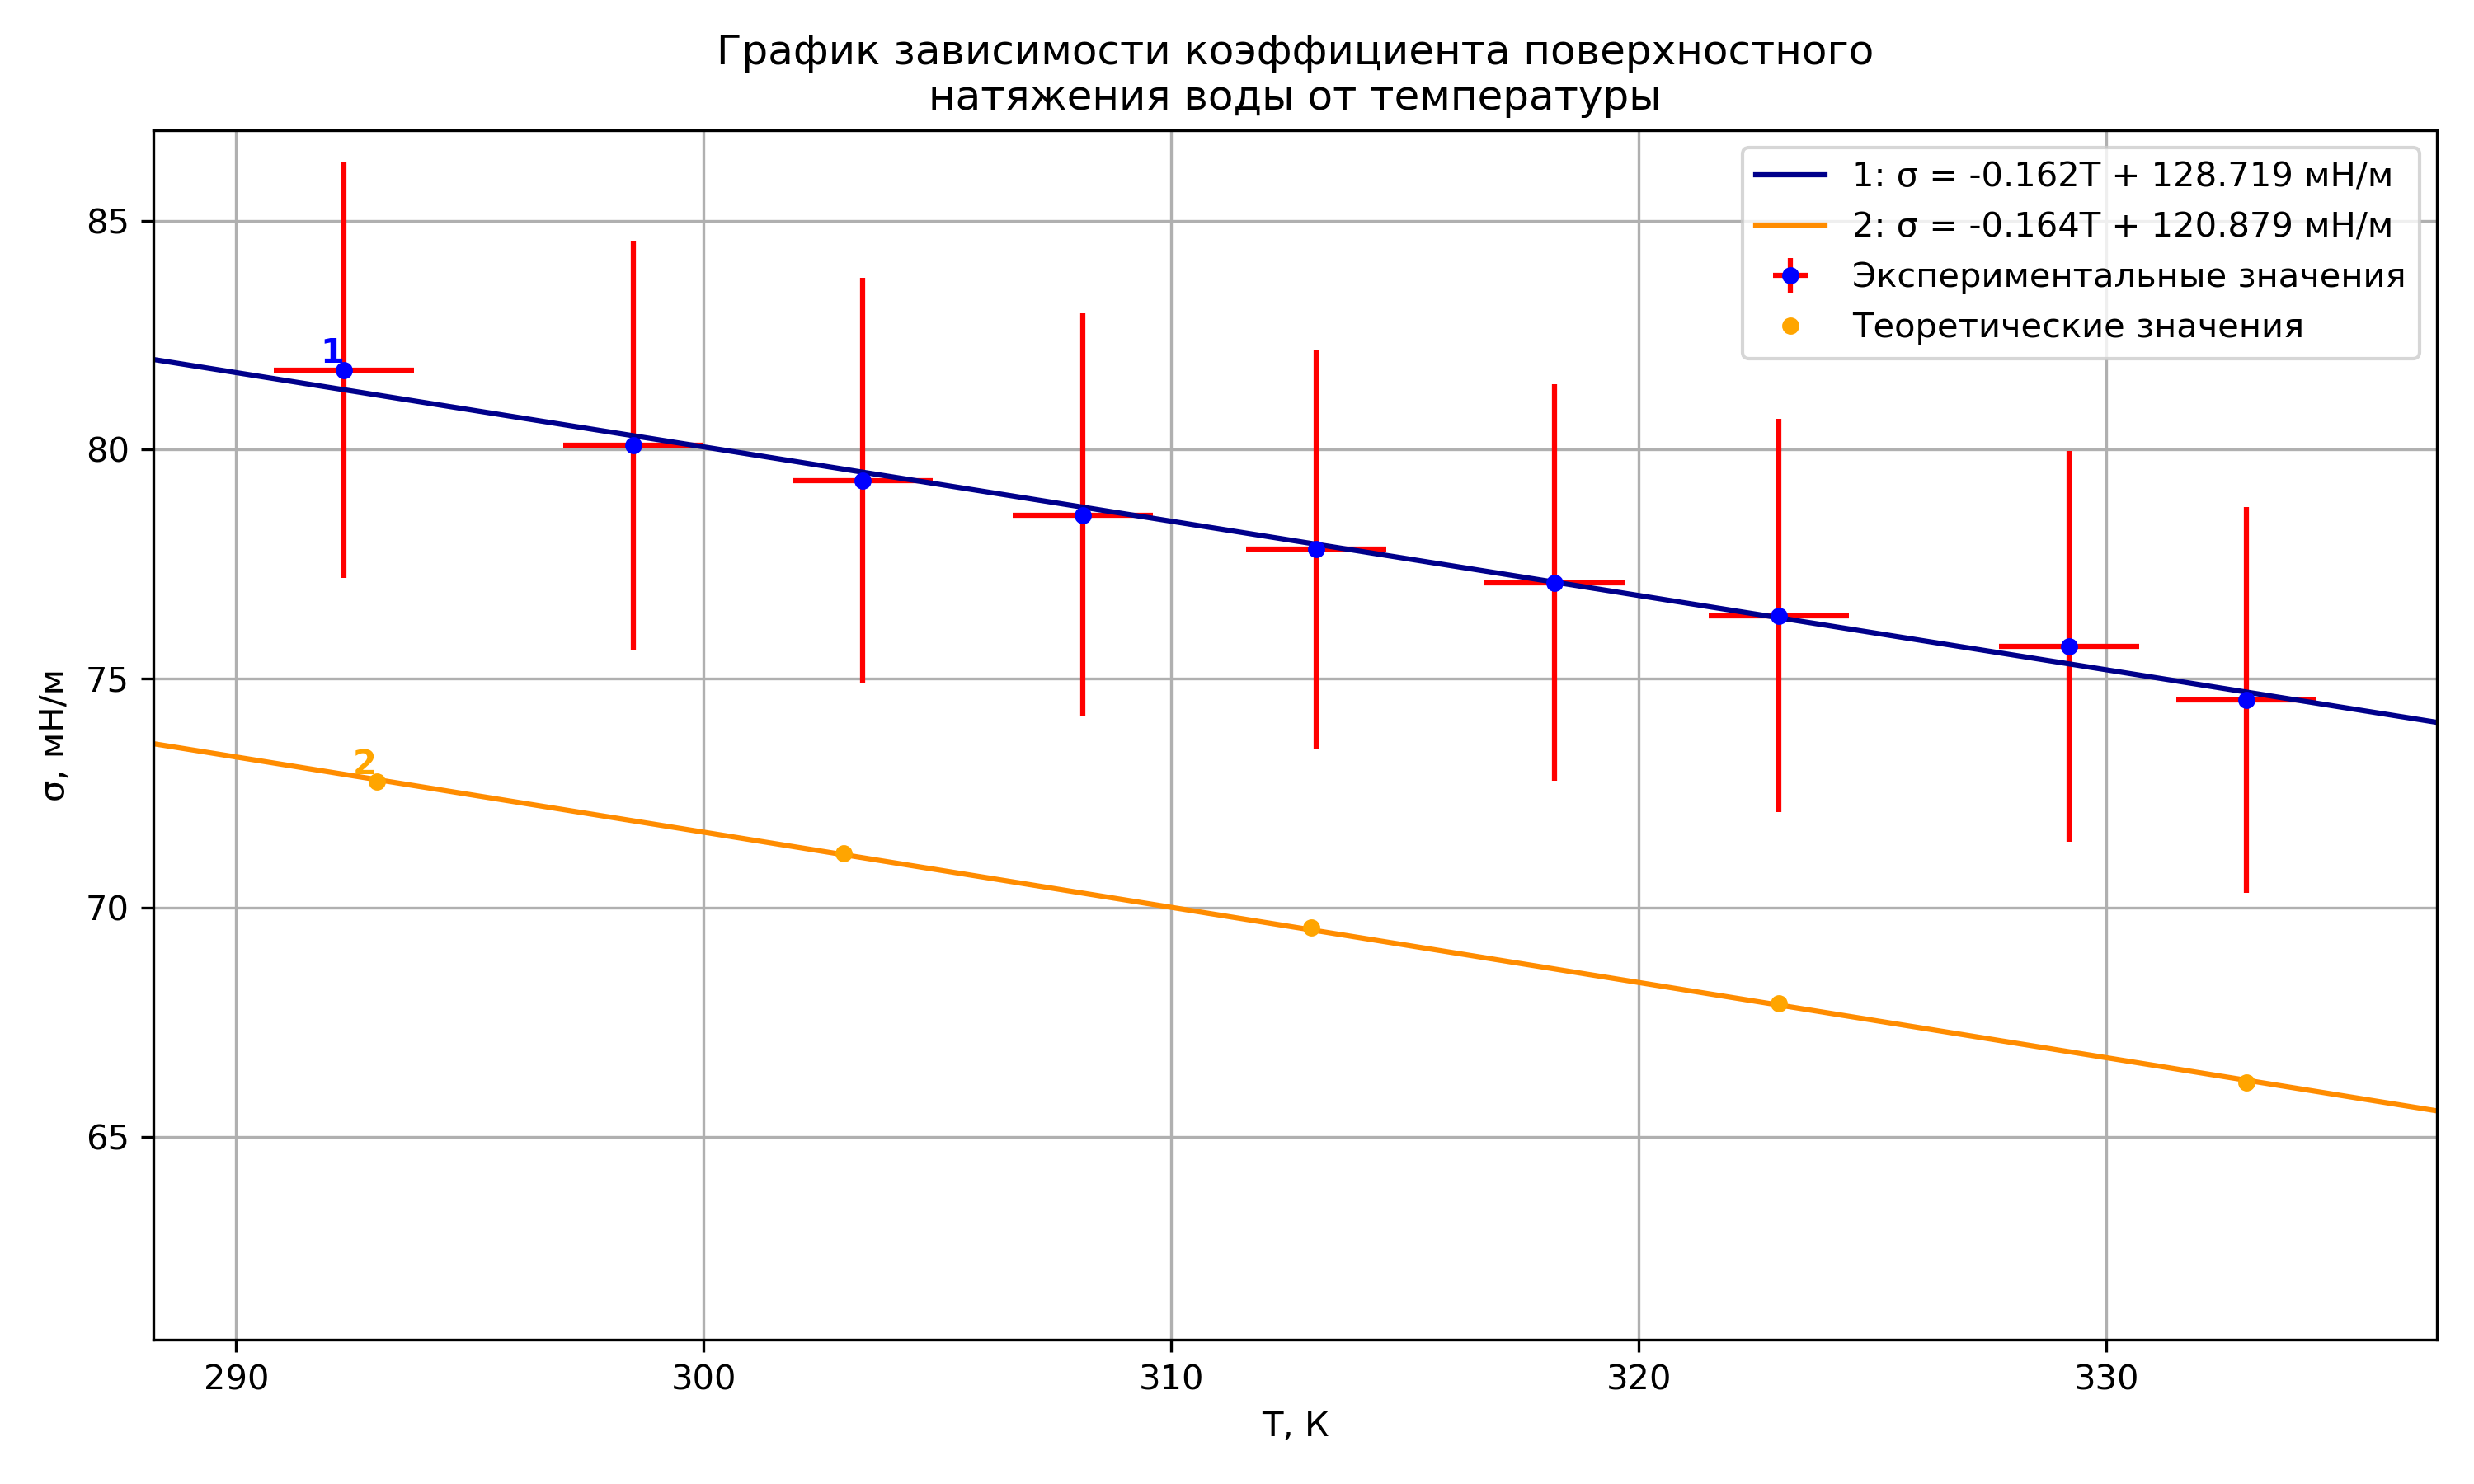
\includegraphics[width=1\textwidth]{Graphics/graph1.png}}
\caption[]{\label{} График №1 Зависимость $\sigma (T)$}
\end{figure}

Температурный коэффициент $\frac{d\sigma}{dT}^{\text{эксп}} = -0,162 \pm 0,062 \frac{\text{мН}}{\text{м} \cdot K}(\varepsilon = 38,8\%)$. Высокая погрешность связана опять же с отличающейся температурой иглы, а также с неустановившейся нужной температурой системы, т.к. для этого требуется больше времени (мы ждали по 5 минут для каждой температуры). На графике также отмечены точки, соответствующие табличным значениям коэффициента. Построив по МНК прямую, получим, что $\frac{d\sigma}{dT}^{\text{теор}} = -0,164 \pm 0,067 \frac{\text{мН}}{\text{м} \cdot K}(\varepsilon = 40,7\%)$.\\
Обратившись к учебнику Кикоиных "Молекулярная физика", в параграфе 103 можно обнаружить зависимость
\begin{equation*}
	\frac{d\sigma}{dT} = -B(\frac{\rho}{\mu})^{\frac{2}{3}},
\end{equation*}
где $B$ - постоянный коэффициент, равный 2,1 в СГС, $\mu$ - молекулярный вес жидкости. Отмечается приближенный характер этой формулы, однако экспериментально она проявляет себя с высокой точностью. С ее помощью даже считают молекулярный вес.\newline

\item Построим график зависимости теплоты образования единицы поверхности жидкости $q  = -T\frac{d\sigma}{dT} $  и поверхностной энергии $U$ единицы площади $\Pi$: $\frac{U}{\Pi} = (\sigma - T\frac{d\sigma}{dT}$) от температуры для наших значений температуры и коэффициентов поверхностного натяжения.\\
\begin{figure}[h!]
\centering{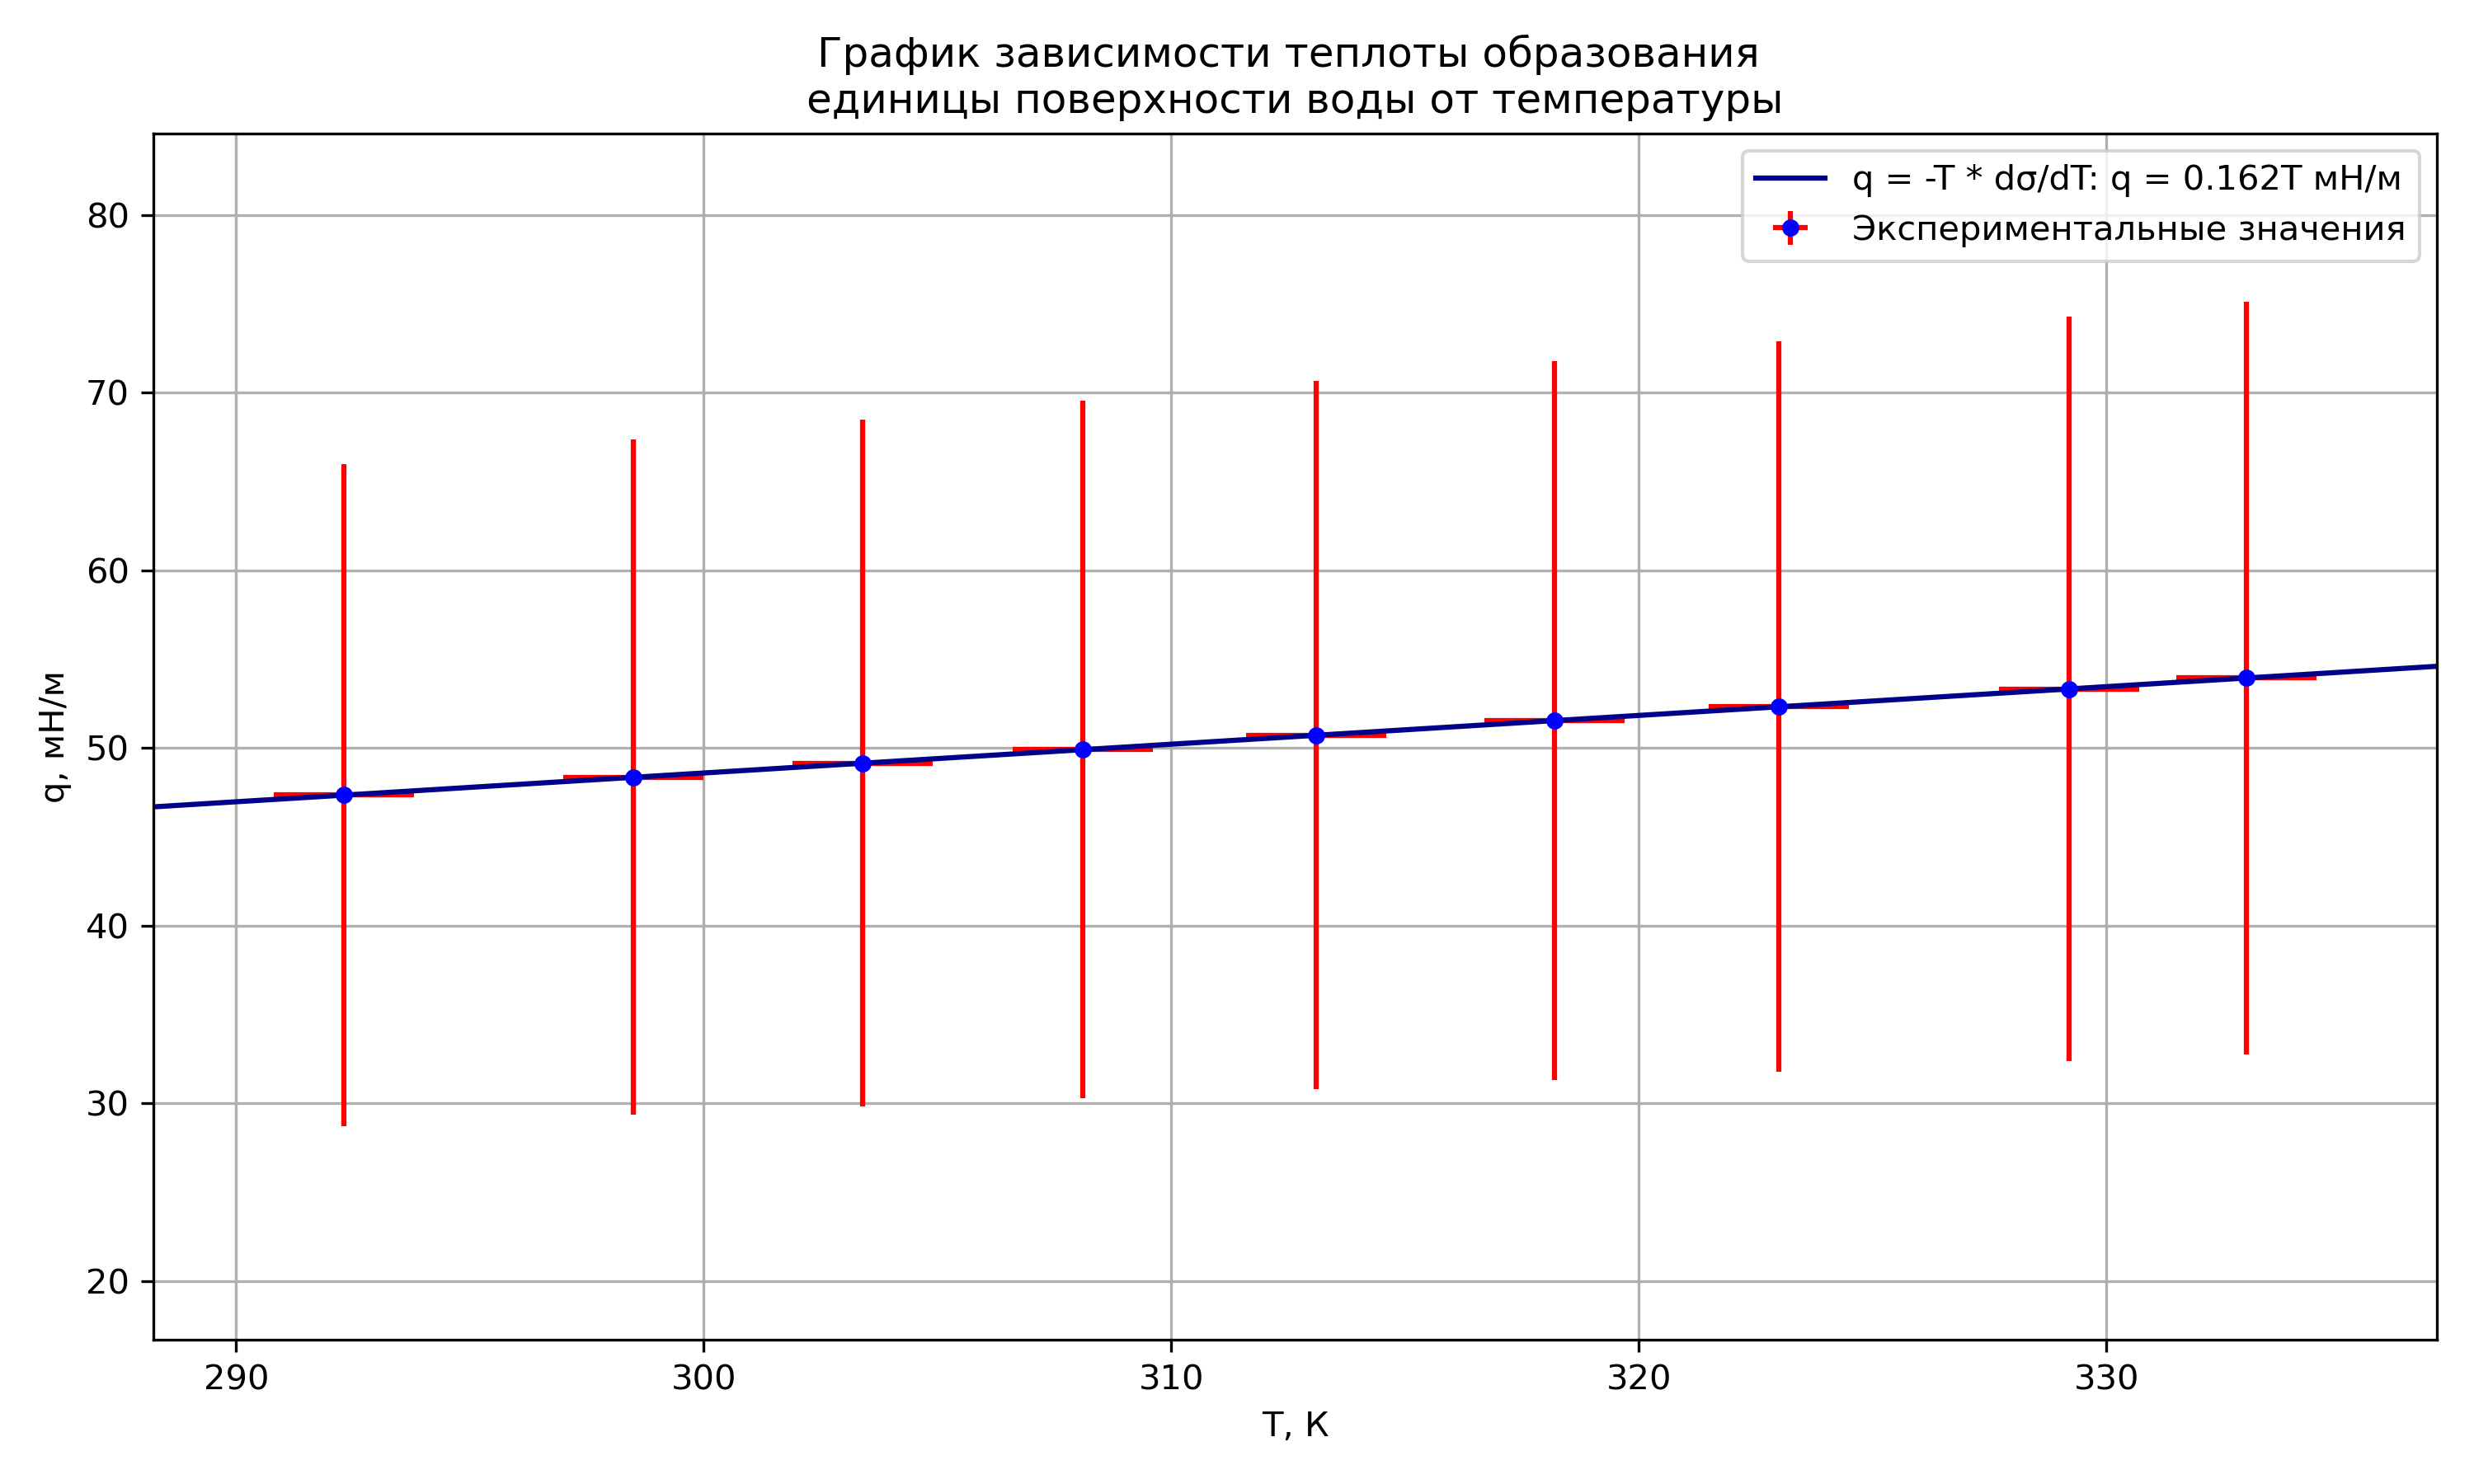
\includegraphics[width=0.8\textwidth]{Graphics/graph2.png}}
\caption[]{\label{} График №2 Зависимость $q(T)$}
\end{figure}

\begin{figure}[h!]
\centering{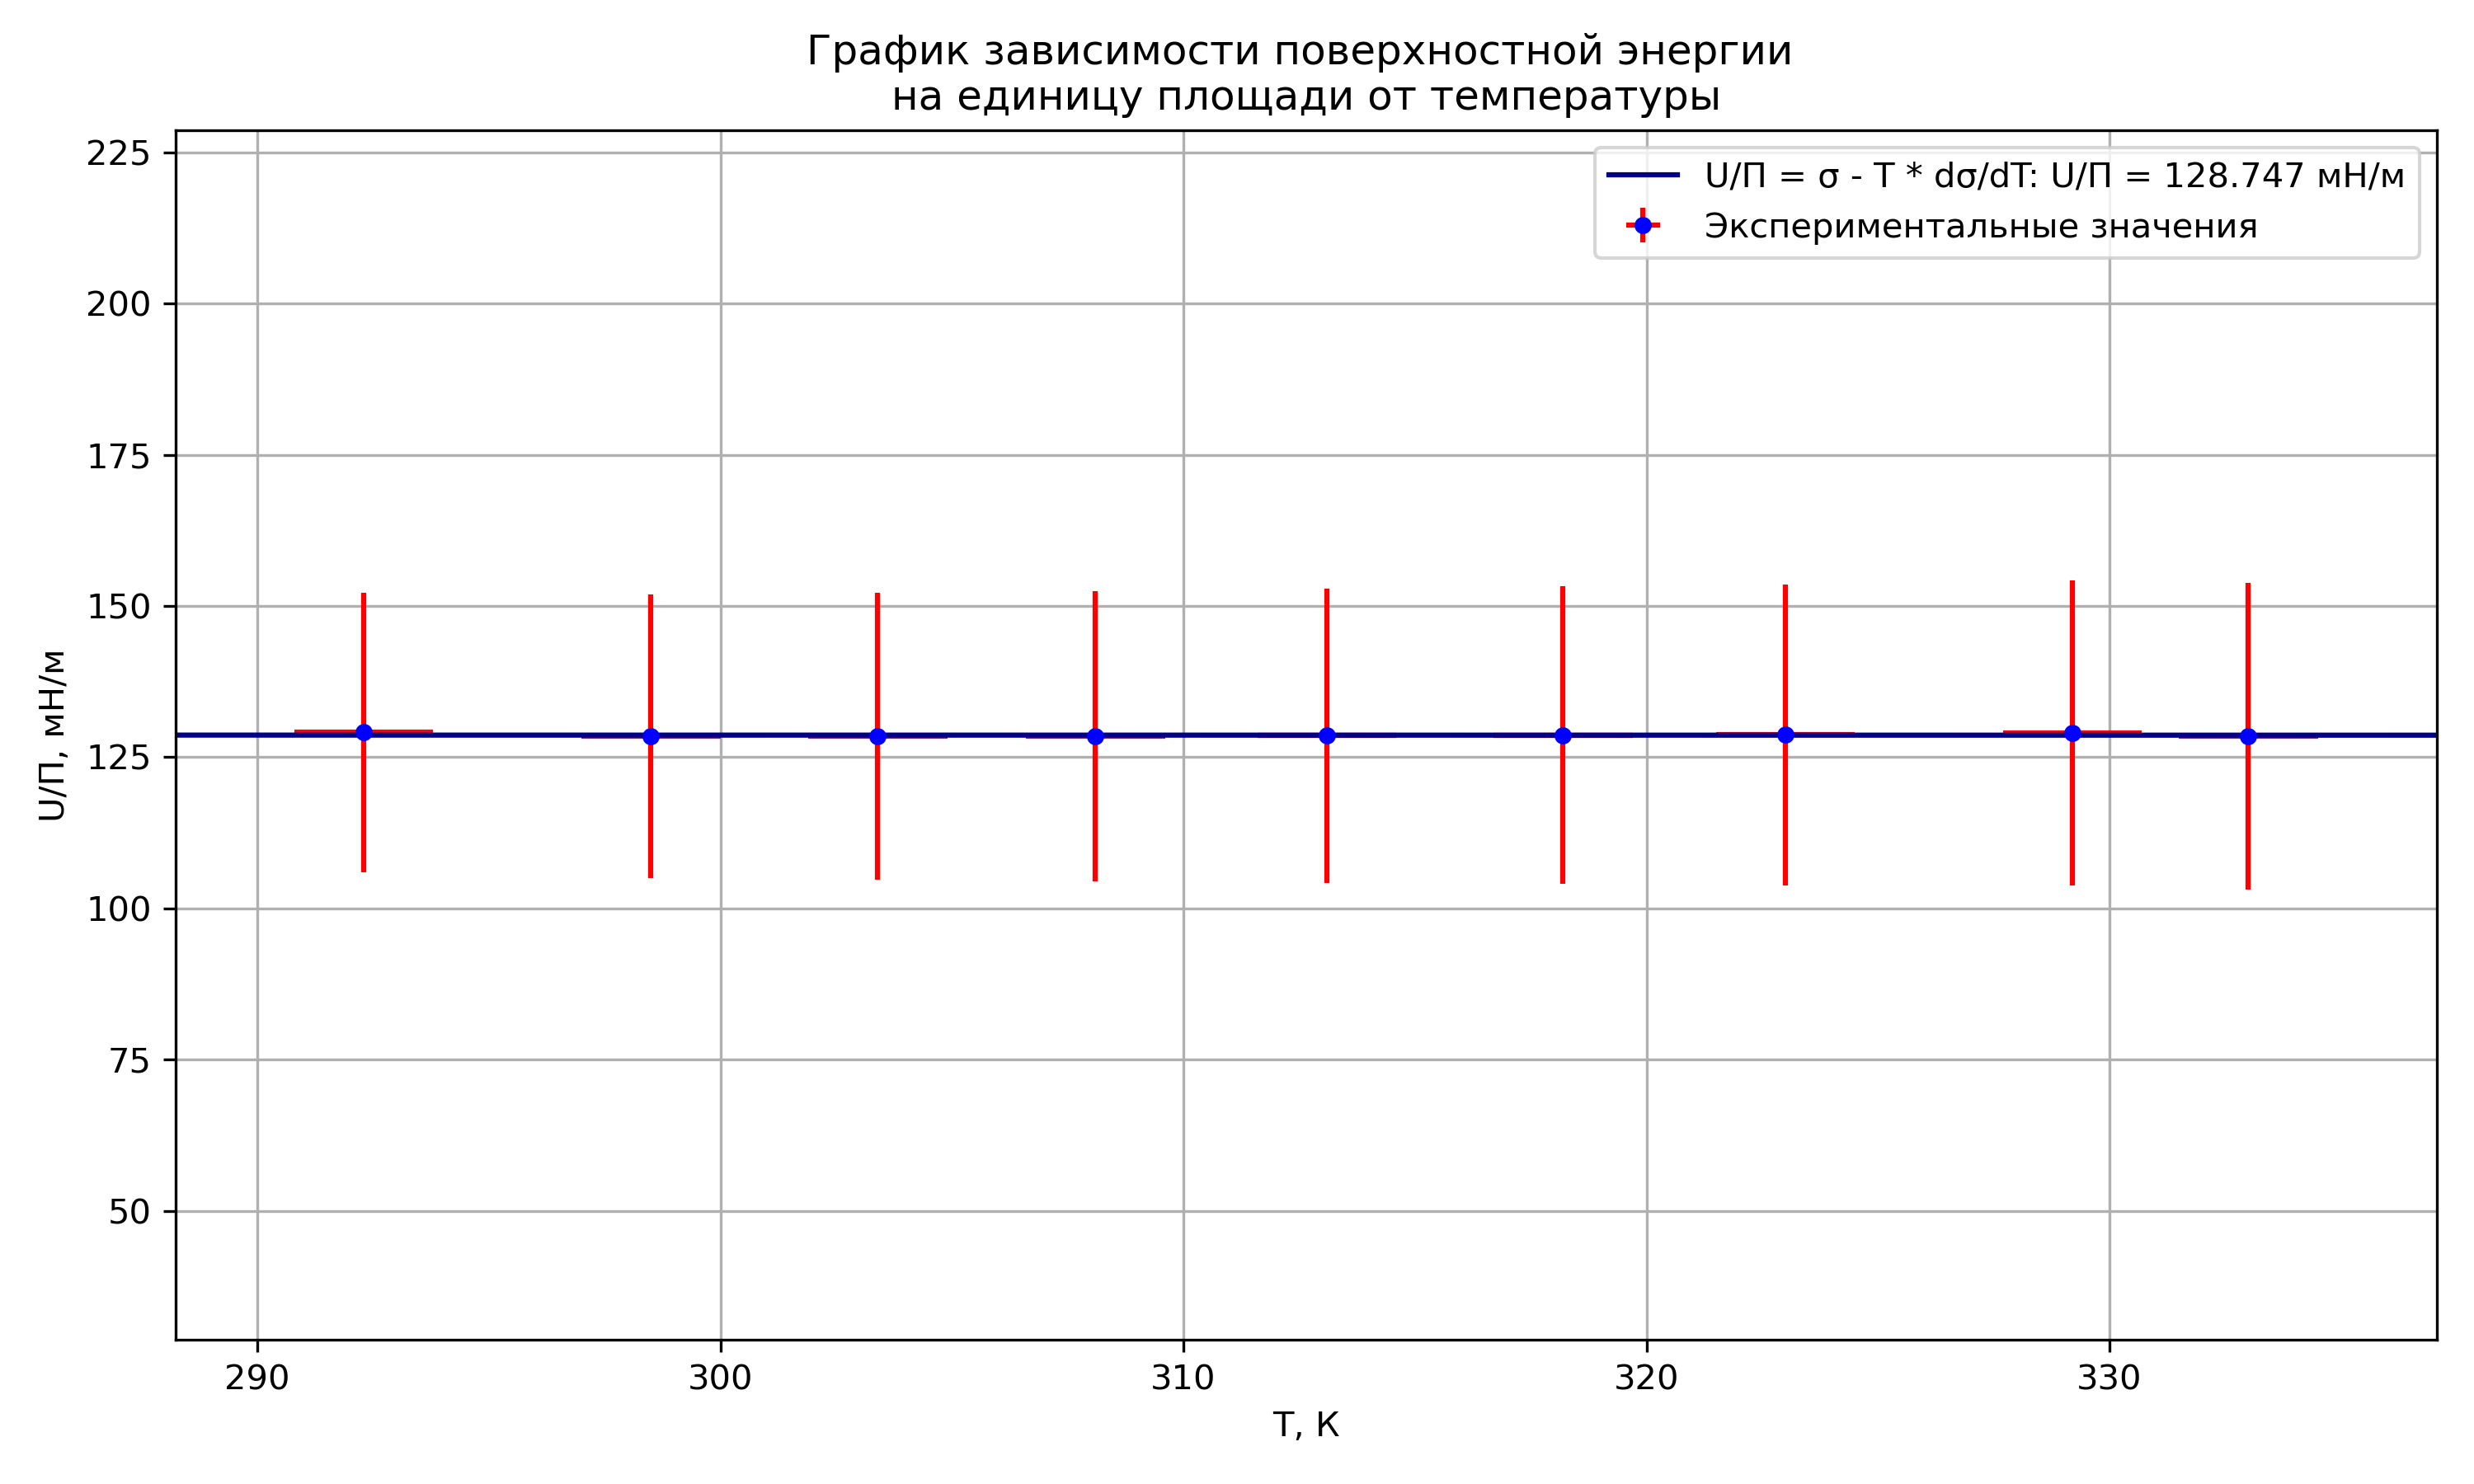
\includegraphics[width=0.8\textwidth]{Graphics/graph3.png}}
\caption[]{\label{} График №3 Зависимость $\frac{U}{\Pi}(T)$}
\end{figure}
\end{enumerate}
\clearpage
\section{Результаты и обсуждения}
Проведя серию измерений разницы давлений от температуры, мы получили следующие значения коэффициентов поверхностного натяжения:\newline

\begin{table}[h!] 
	\caption{Таблица №5 Сравнение табличных и экспериментальных значений коэффициентов поверхностного натяжения воды}
	\begin{center}
		\begin{tabular}{|*{7}{c|}}
			\hline
			 $T$, K & $\sigma^{\text{эксп}}$, $\frac{\text{мН}}{\text{м}}$ & $\sigma^{\text{табл}}$, $\frac{\text{мН}}{\text{м}}$ & $\Delta \sigma^{\text{эксп}}$, $\frac{\text{мН}}{\text{м}}$ & $\Delta \sigma^{\text{табл}}$, $\frac{\text{мН}}{\text{м}}$ & $\varepsilon_{\text{эксп}}$, \% & $\varepsilon_{\text{табл}}$, \%\\ \hline
			$292,3\pm 1,5$& 81,74&	72,86&	4,54&	8,89&	5,55&	12,20\\ \hline
			$298,5\pm 1,5$& 80,09&	71,88&	4,47&	8,20&	5,58&	11,42\\ \hline
			$303,4\pm 1,5$& 79,32&	71,12&	4,43&	8,21&	5,59&	11,54\\ \hline
			$308,1\pm 1,5$&78,57&	70,35&	4,40&	8,22&	5,60&	11,68\\ \hline
			$313,1\pm 1,5$& 77,83&	69,54&	4,36&	8,28&	5,61&	11,91\\ \hline
			$318,2\pm 1,5$& 77,01&	68,70&	4,33&	8,40&	5,60&	12,22\\ \hline
			$323,0\pm 1,5$& 76,38&	67,91&	4,30&	8,47&	5,63&	12,47\\ \hline
			$329,2\pm 1,5$& 75,71&	66,84&	4,27&	8,87&	5,64&	13,27\\ \hline
			$333,0\pm 1,5$& 74,53&	66,18&	4,21&	8,35&	5,65&	12,61\\ \hline
		\end{tabular}
	\end{center}
\end{table}
Данные табличных коэффициентов были взяты изкниги Лабораторный практикум по общей физике Том 1 Термодинамика и молекулярная физика и рассчитаны с учетом линейной аппроксимации. Т.е. если температура $T$ лежит в пределах ближайших температур в таблице $T_1$ и $T_2$, то $\sigma = \sigma_1 + \frac{\sigma_2 - \sigma_1}{T_2 - T_1}(T - T_1)$
Погрешность коэффициента обусловлена загрязнением оборудования (иглы, трубок), неравновесностью системы, погрешностью оборудования и случайными погрешностями эксперимента.
\section{Выводы}
В данной работе проведено измерение диаметра иглы с помощью известного коэффициента поверхностного натяжения спирта. $d_{\text{иглы}}^{exp} =0,915 \pm 0,055 \text{ мм }(\varepsilon_{d} = 6,0\%)$. Также диаметр был измерен с помощью микроскопа, $d = 1,10 \pm 0,05 \text{ мм}$ ($\varepsilon = 4,5\%$). Погрешность измерения с помощью микроскопа меньше, поэтому в дальнейшем мы использовали именно это значение.
Проверили установку, измерив разницу высот столбов исследуемой жидкости и вычислив по разнице давлений. $\Delta H^{real} = H_1 - H_2 = 1,60 \pm 0,05 \text{ см}$, $\Delta H^{exp} =  0,94 \pm 0,12 \text{ см}(\varepsilon = 13,1 \%)$. Большая разница обусловлена загрязнением оборудования.
Получили значения коэффициентов поверхностного натяжения дистиллированной воды при различных температурах, сравнили с табличными (см. таблицу №5).
Определили полную поверхностную энергию и теплоту, необходимую для изотермического образования единицы поверхности жидкости  при различной температуре. Убедились, что с ростом температуры коэффициент поверхностного натяжения уменьшается, теплота увеличивается, а полная поверхностная энергия не меняется. Высокая погрешность величин обусловлена тем, что для установления теплового равновесия требуется больше времени (более 5 минут), чем мы ждали, а также погрешностью приборов. 


\end{document}